\section{The attribution ladder}
\label{sec:attribution}

\begin{definition}[Rungs and shares]
\label{def:ladder}
For a model $m$ evaluated on the same structures, let
$R_0 = \tfrac{1}{n}\sum \mathbf{1}[\spg(s) = y(s)]$ (the symmetry algorithm on ground-truth positions),
$R_1$ the oracle ceiling of Definition~\ref{def:ceiling},
$R_3(m)$ the accuracy of $m$ given ground-truth fractional coordinates, species and cell parameters as
text, and
$R_4(m)$ the accuracy of $m$ on the pixel renders. Define the \emph{perception component}
$P(m) = R_3(m) - R_4(m)$, the \emph{symbolic residual} $S(m) = R_1 - R_3(m)$, and the \emph{perception
share} $P(m) / (R_1 - R_4(m))$. $R_2$ denotes the oracle run on a learned detector's output.
\end{definition}

Three conditions make the shares interpretable, and we state them because each is checkable: the rungs are
scored on the same named structures with all comparisons paired; $R_3$ and $R_4$ use the same decode budget
($K{=}3$ everywhere the shares are computed); and the symbolic residual \emph{bounds} rather than isolates
symmetry reasoning, since a residual against a deterministic solver can include failure modes other than
symmetry (we test this directly below). Table~\ref{tab:rungs} gives the ladder.

\begin{table}[t]
\centering
\caption{Attribution ladder, original evaluation sample, $n=210$, $K{=}3$. The two model columns are the
strongest scored model and one mid-roster model, named rather than aggregated; $R_3$ and $R_4$ within
a column are the same model under two conditions, so their interval is that model's perception component
(Definition~\ref{def:ladder}). $R_2$ is unscored: its extractor fails to triangulate on 19.0\% and 22.4\%
of structures, over the pre-registered 5\% gate. The fine-tuned arm was never run under the coordinate
condition, so it carries no within-model interval and is not a column.}
\label{tab:rungs}
\small
\setlength{\tabcolsep}{4.5pt}
\begin{tabular}{p{0.40\linewidth}p{0.22\linewidth}rr}
\toprule
rung & what it removes & \small gemini-3.6-flash & \small gpt-4.1-mini \\
\midrule
$R_0$ algorithm on ground-truth positions & nothing & \multicolumn{2}{c}{1.0000 (definitional)} \\
$R_1$ oracle: camera inversion, then algorithm & the protocol's losses & \multicolumn{2}{c}{0.9524} \\
$R_3$ exact geometry as text ($K{=}3$) & the model's perception & 0.8524 & 0.4143 \\
$R_4$ pixels ($K{=}3$) & nothing further & 0.7333 & 0.3667 \\
\midrule
perception share $(R_3-R_4)/(R_1-R_4)$ & --- & 0.5436 & 0.0813 \\
$R_2$ oracle on a learned detector's output & ideal extraction & \multicolumn{2}{c}{unscored} \\
\bottomrule
\end{tabular}
\end{table}

\textbf{The top rung is definitional, and that is load-bearing.} The label \emph{is} $\spg$ applied to the
structure, so $R_0 = 1.0000$ exactly, and the $R_0 \to R_1$ interval is what camera inversion and
correspondence re-solution cost. Treating $R_0$ as approximately equal to $R_1$ would discard that
interval.

\textbf{Exact geometry does not close the gap.} Supplying ground-truth geometry as text (the CIF-supplied
condition of \citet{xcrys2506}, cited as prior use) lifts every model substantially, and none reaches the
oracle: the best is 0.8524 against 0.9524. The pre-registered decomposition of Definition~\ref{def:ladder}
gives a median perception share of 30.9\% across the 14 models scored under the coordinate condition, with
the symbolic residual the larger of the two for 12 of them; the two columns of Table~\ref{tab:rungs} differ
in perception share by a factor of six. Only the two strongest models are perception-dominated, and the
share tracks pixel accuracy (Spearman $\rho = -0.6439$, $p = 0.0130$). \emph{The bottleneck moves with
model strength}: a more precise statement than either single attribution, and one visible only because the
oracle fixes the top of the ladder.

\textbf{A control pair makes $R_3$ readable.} Removing the images and leaving only the chemical formula
collapses every scored model toward seven-way chance (mean 0.1487 over the 13 models scored under the
image-removal control). Removing the images and supplying full geometry lifts every scored model to
between 0.4143 and 0.8524.
The two conditions differ in one thing, so the lift is the geometry rather than text-mode prompting; the
geometry prompts are also shorter than the five-image prompts they beat, which rules out a length artefact.

\textbf{The symbolic residual is an upper bound, and we tested it.} A residual against a solver may include
long-list handling rather than symmetry reasoning. Regressing per-structure $R_3$ correctness on
conventional-cell atom count over the same records (no new model calls): pooled over the 14 scored models
and 2940 model-structure pairs, Spearman $\rho = -0.0908$ at $p = 8.1\times10^{-7}$; 13 of 14 models are
negative, and accuracy falls from 0.5551 on cells at or below the median 14 atoms to 0.5129 above it
(Fisher $p = 0.0241$). The pre-registered confound control does not rescue it: atom count correlates with
crystal system ($\rho = -0.1866$), but the mean within-system association is $-0.1053$, stronger than the
pooled figure rather than attenuated, so the effect is not symmetry difficulty in disguise. We therefore
report the symbolic residual as an upper bound on a symmetry-reasoning deficit, not as a measurement of
one. Nothing here touches the oracle-to-model gap, which is measured against pixels.

\textbf{A learned extractor fabricates its output.} Substituting a strong model as the extraction stage,
prompted for species and positions with the symmetry question withheld, and having a weaker model answer
from that text yields 0.1429. That arm predicted two of seven classes and its accuracy equals the majority
stratum's base rate, so it measures nothing. The informative measurement is the intermediate, scored
directly against ground truth: median recall 0.0000, with 105 of 206 structures having not one emitted atom
within tolerance of a real one, despite a median of 48 well-formed atoms per structure. A colour-threshold
blob detector achieves median recall 0.400 on the same task. Downstream accuracy alone would have read this
as bad reasoning. \emph{A two-stage pipeline whose intermediate cannot be checked will attribute
fabrication to reasoning}, which is the argument for the instrument.

\begin{figure}[t]
\centering
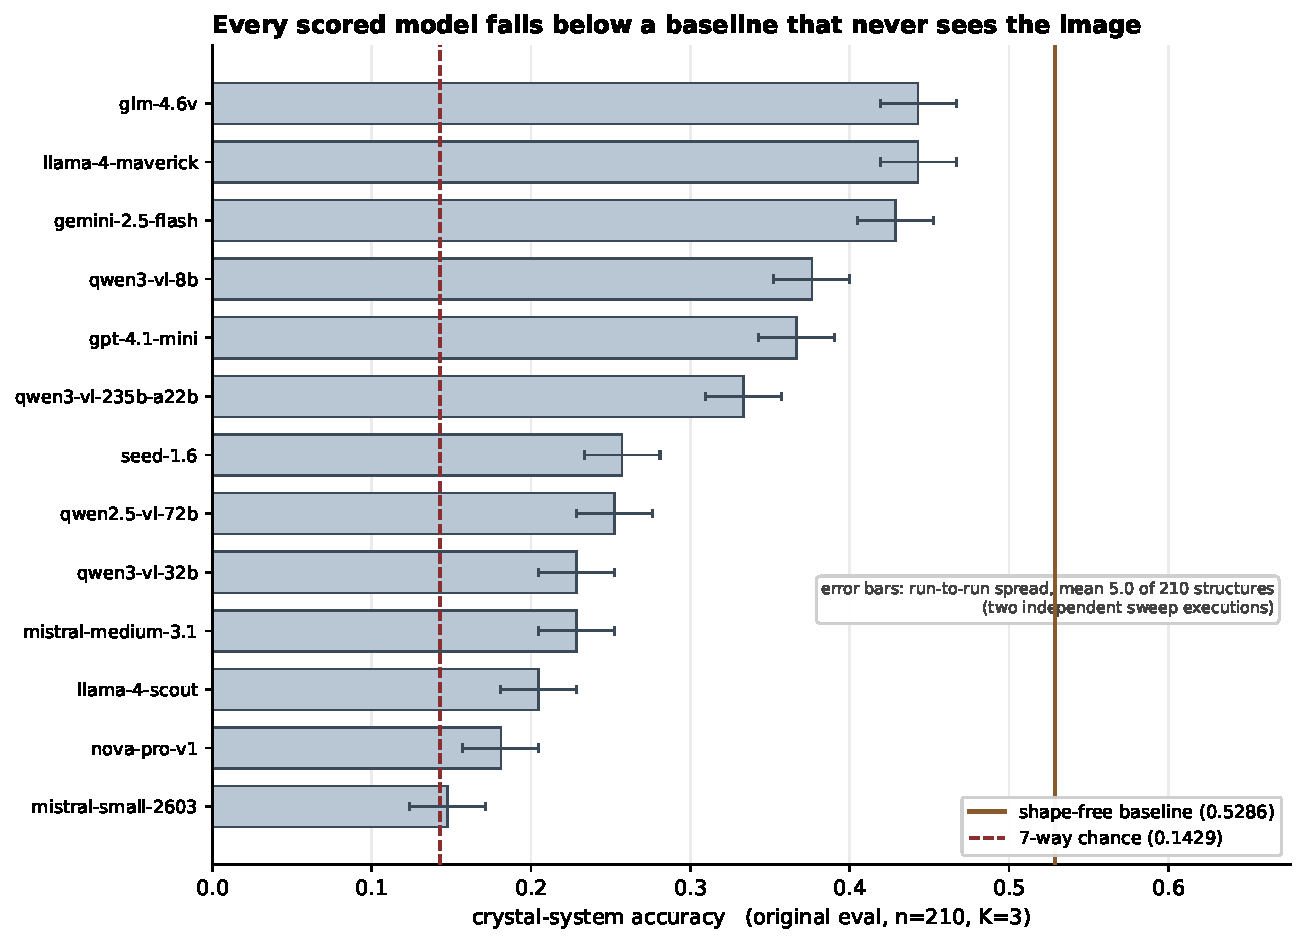
\includegraphics[width=0.8\linewidth]{figures/leaderboard.pdf}
\caption{Zero-shot leaderboard, original sample, $n=210$, $K=3$, 13 scored models across eight vendors.
Dashed line: the shape-free baseline (atom count, density, cell volume) on this sample. Error bars: the
measured run-to-run spread of $K{=}3$ majority voting.}
\label{fig:leaderboard}
\end{figure}
